\subsection{ResNet}
\begin{frame}{}
    \LARGE CNN Architectures: \textbf{ResNet}
\end{frame}

% ResNet
\begin{frame}{ResNet: Motivation}
    \begin{itemize}
        \item \textbf{Problem:} Making networks deeper does not always improve accuracy.
        \item \textbf{Why?} In very deep networks, gradients become extremely small as they move backward through layers, making learning slow or stopping it altogether (\textbf{vanishing gradient problem}).
        \item \textbf{Solution:} Residual Network (ResNet) introduces \textbf{skip connections (residuals)}, allowing information to flow more easily.
    \end{itemize}
\end{frame}

\begin{frame}{ResNet}
    \begin{itemize}
        \item Very deep networks using residual connections
        \item 152-layer model for ImageNet
        \item Stacked Residual Blocks
        \item \textbf{Residual:} A shortcut connection that helps the network pass information through layers more easily.
    \end{itemize}

    \begin{figure}
        \centering
        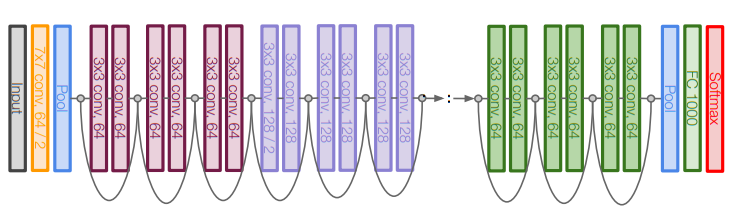
\includegraphics[width=1.0\textwidth,height=0.6\textheight,keepaspectratio]{images/cnn/resnet_1.png}
    \end{figure}
\end{frame}

\begin{frame}{ResNet}
    \begin{itemize}
        \item What happens when we continue stacking deeper layers on a "plain" convolutional neural network?
    \end{itemize}
\pause
    \begin{figure}
        \centering
        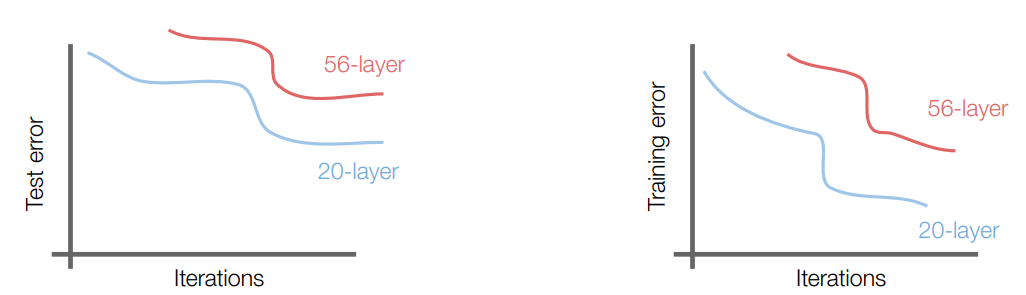
\includegraphics[width=1.0\textwidth,height=0.5\textheight,keepaspectratio]{images/cnn/resnet_2.png}
    \end{figure}

\pause
    \begin{itemize}
        \item 56-layer model performs worse on both test and training error
        \pause
        \item The deeper model performs worse, but it’s not caused by overfitting!
    \end{itemize}
\end{frame}


\begin{frame}{ResNet}
    \begin{itemize}
        \item \textbf{Fact:} Deep models have more representation power (more parameters) than shallower models.
        \pause
        \item \textbf{Hypothesis:} The problem is an optimization problem, deeper models are harder to optimize
        \pause
        \item \textbf{Solution:} Use network layers to fit a residual mapping instead of directly trying to fit a desired underlying mapping
    \end{itemize}
\pause
    \begin{figure}
        \centering
        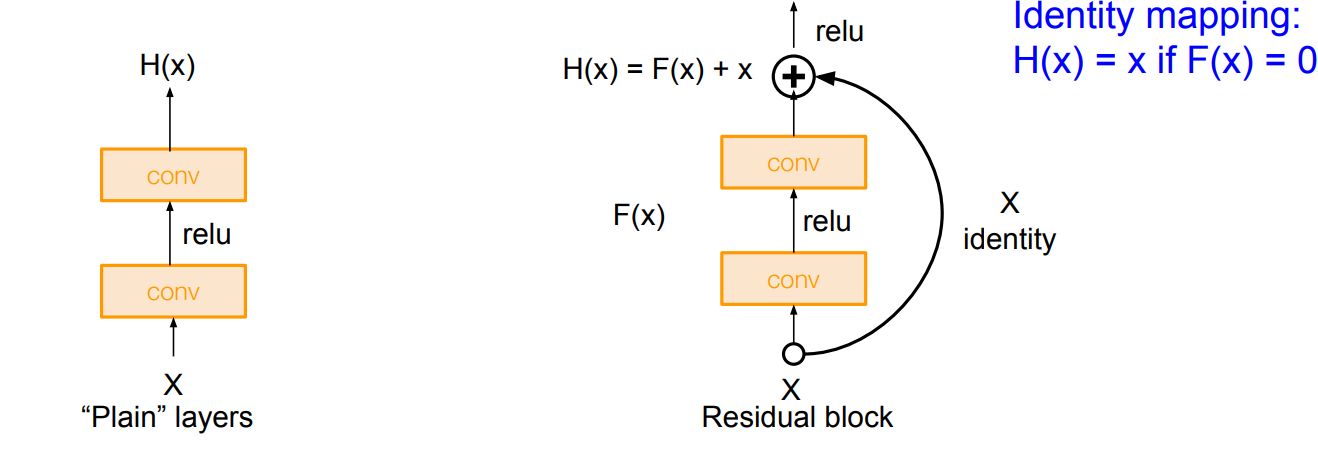
\includegraphics[width=1.0\textwidth,height=0.5\textheight,keepaspectratio]{images/cnn/resnet_3.png}
    \end{figure}
\end{frame}